\documentclass[11pt]{article}

\usepackage{natbib,rotfloat,epsfig,setspace,amssymb,amsmath, comment}

\setlength{\hoffset}{0.01in}
\setlength{\voffset}{-0.6in}
\setlength{\textwidth}{6.0in}
\setlength{\evensidemargin}{0in}
\setlength{\oddsidemargin}{0in}
\setlength{\textheight}{8.5in}

\begin{document}

\onehalfspace

\title{Economics 512 -- Homework 6}
\author{Maxence Valentin}
\date{January 23, 2019}
\maketitle

\paragraph{Question 1.}

Given a stock of unharvested wood k and price p at time t, the firm's dynamic problem can be summarized as:
\begin{equation*}
\begin{aligned}
& \underset{x\in[0,k]}{\text{max}} 
& & p_tx - 0.2x^{1.5} + \delta E[V(p_{t+1},k_{k+1})|p_t] \\
& \text{subject to}
& &  k_{t+1} = k - x
\end{aligned}
\end{equation*}
where x is the harvested stock at period t and V(p,k) is the value function. By Bellman principle of optimality and by letting k' to be the stock available at period t+1, the firm's problem would be summarized as:
\begin{equation}
	V(p,k)= \max_{k'\in[0,k]} \pi (k',p) + \delta E[V(p',k')|p] 
\end{equation}

The state variables are the current stock and current price. Stock transition is deterministic while price follow an AR(1) process $p_{t+1} = p_0 + \rho p_t + u_{t+1}$. The policy variable is consumption x (or next period stock k'=k-x). 


\paragraph{Question 2.} See attached code. The 21 grids points span the [0.65;1.35] price space. The stock (current and remaining) is assumed to take only integers value from 0 to 100. 

\paragraph{Question 3-5.} See attached code and figure 1 through 4.

\begin{figure}[!h]
	\centering
	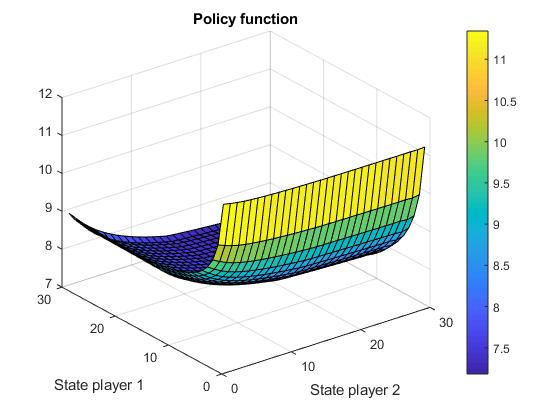
\includegraphics[width=0.8\textwidth]{Figures/figure1.jpg}
	\caption{Question 3}
\end{figure}

\begin{figure}[!h]
	\centering
	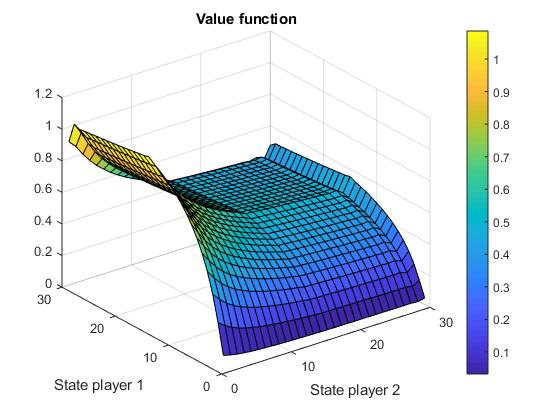
\includegraphics[width=0.8\textwidth]{Figures/figure2.jpg}
	\caption{Question 4}
\end{figure}

\begin{figure}[!h]
	\centering
	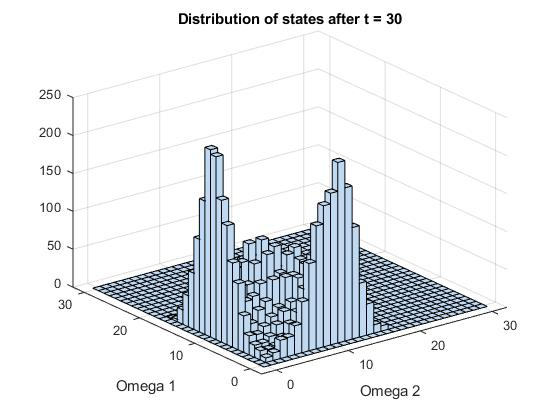
\includegraphics[width=0.8\textwidth]{Figures/figure5.jpg}
	\caption{Question 5a}
\end{figure}

\begin{figure}[!h]
	\centering
	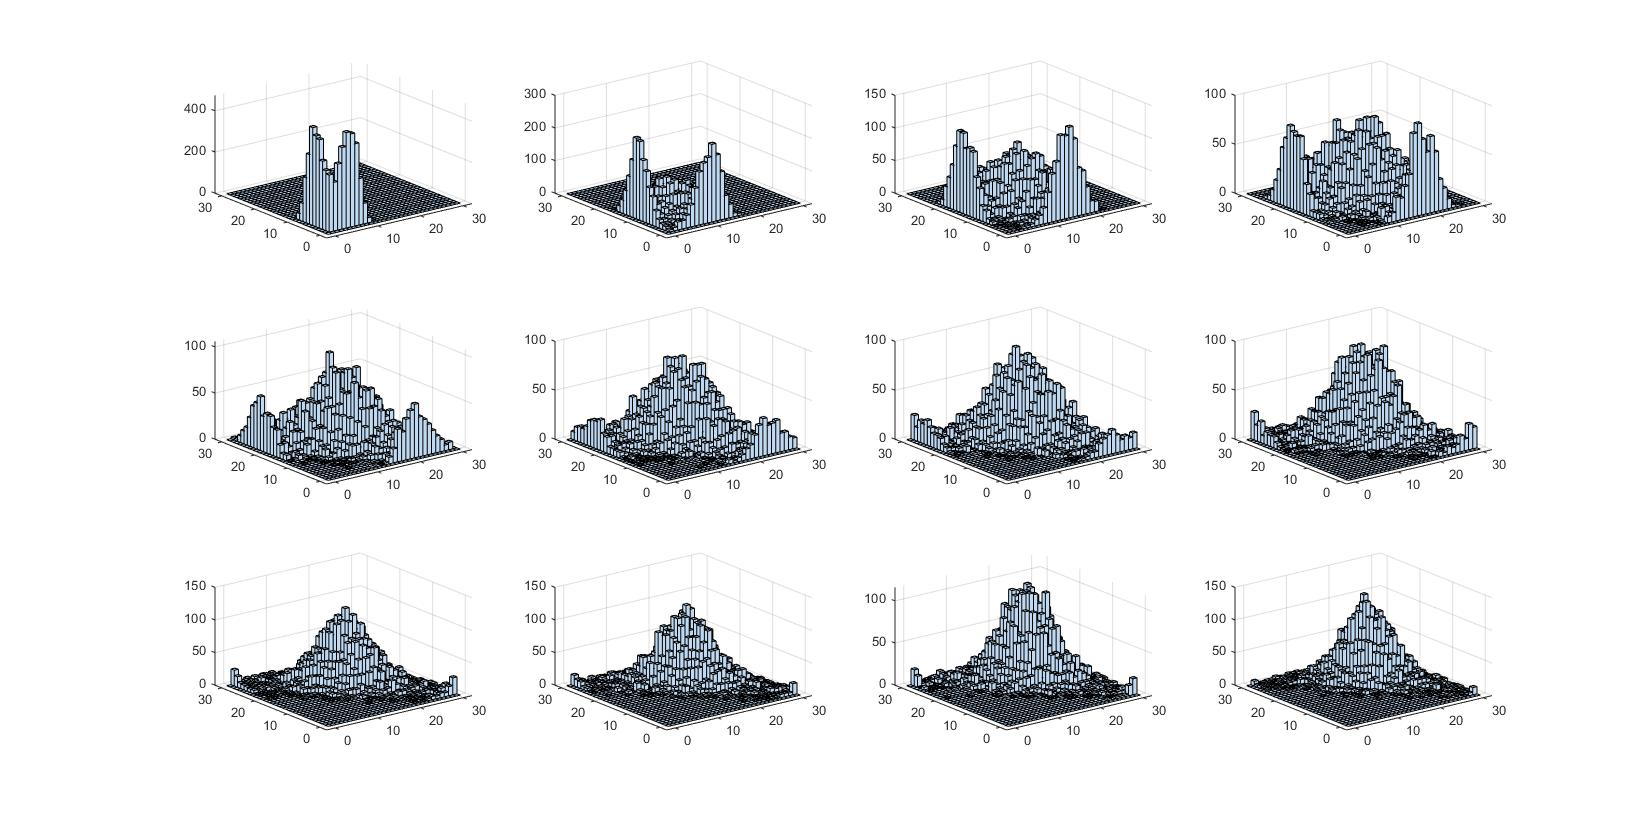
\includegraphics[width=0.8\textwidth]{Figures/figure6.jpg}
	\caption{Question 5b}
\end{figure}



\paragraph{Question 6.} Changing the grid representation in the price space. See code and Figure 5 and 6.


\begin{figure}[!h]
	\centering
	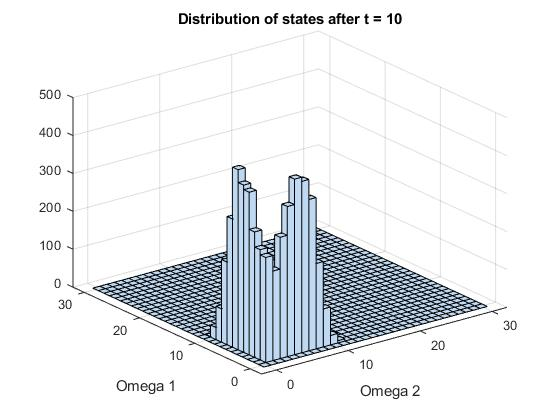
\includegraphics[width=0.8\textwidth]{Figures/figure3.jpg}
	\caption{Question 6a}
\end{figure}

\begin{figure}[!h]
	\centering
	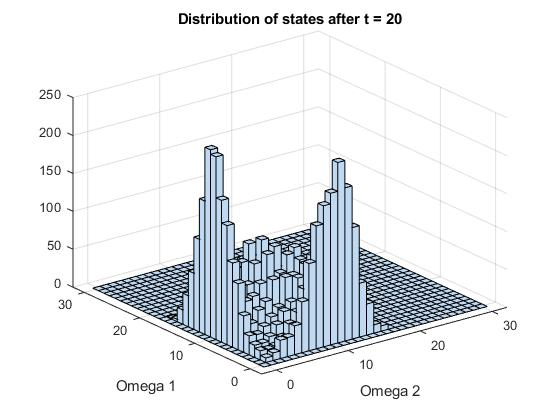
\includegraphics[width=0.8\textwidth]{Figures/figure4.jpg}
	\caption{Question 6b}
\end{figure}




\end{document}
